\label{sec:background}
\subsection{CNN based methods in DSLAM}
As described before, there are two essential components on each agent: 1) Visual Odometr(VO) and 2) Place Recognition.

\subsection{Hardware architecture of Zync SoC}
The Xilinx Zync Soc is a chip with ARM cores and FPGA fabric. The system is illustrated in \cref{fig:plps}. The ARM cores with an embedded Linux operation system are called Processing System (PS). The FPGA fabric is called Programmable Logic (PL). The peripherals like camera and communication unit (WiFi or others) are accessable with PS. The high-bandwidth on-chip AXI interface is used to communicate between PS and PL. PS and PL can also share the DDR to transfer large volume of data such as each frame of camera.

\begin{figure}[thb]  
    \centering  
    {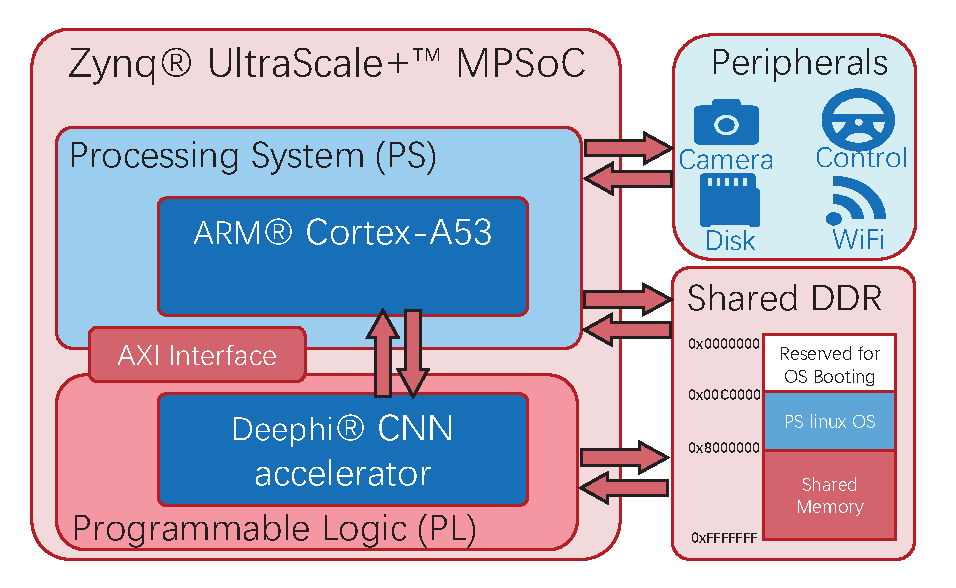
\includegraphics[width=0.95\linewidth]{fig/plps.eps}\label{fig:plps}} 
    \caption{Hardware architecture of Zynq SoC}
\end{figure}